\section{Auswertung}
\label{sec:Auswertung}

\subsection{Bestimmung der Winkelrichtgröße}

Die aufgenommen Messdaten zur Bestimmung der Winkelrichtgröße sind in Tabelle \ref{tab:Messdaten1}
zu finden. Dabei wurde die Kraft bei verschiedenen Auslenkwinkeln $\varphi$ gemessen. Der Hebelarm
hat die konstante Länge \SI{0.3}{\meter}.

\begin{table}
\centering
\caption{Ausgelenkter Winkel mit dazugehöriger Kraft}
\label{tab:Messdaten1}
\sisetup{table-format=2.1}
\begin{tabular}{c c c c}
\toprule
$\text{Winkel} \,/\, °$ & $\text{Winkel} \,/\, \text{rad}$ & $F \,/\, \si{\milli\newton}$ & $M \,/\, \si{\milli\newton\meter}$\\
\midrule
 35 & 0,61 &  30 &  9,00\\
 45 & 0,79 &  35 & 10,05\\
 50 & 0,87 &  40 & 12,00\\
 55 & 0,96 &  50 & 15,00\\
 60 & 1,05 &  55 & 16,50\\
 70 & 1,22 &  61 & 18,30\\
 80 & 1,40 &  83 & 24,90\\
 90 & 1,57 & 102 & 30,60\\
100 & 1,66 & 110 & 32,40\\
 95 & 1,74 & 108 & 33,00\\
\bottomrule
\end{tabular}
\end{table}

Anhand von Formel \eqref{eqn:Winkelrichtgröße} ist zu erkennen, dass die Winkelrichtgröße $D$ 
lediglich ein Proportionalitätsfaktor zwischen Drehmoment $M$ und Winkel $\varphi$ ist. Zur Ermittlung 
dieser Größe wird eine lineare Regression mittels python und matplotlib durchgeführt. 
Das Ergebnis ist in Abbildung \ref{fig:plot1} zu sehen. 


\begin{figure}
  \centering
  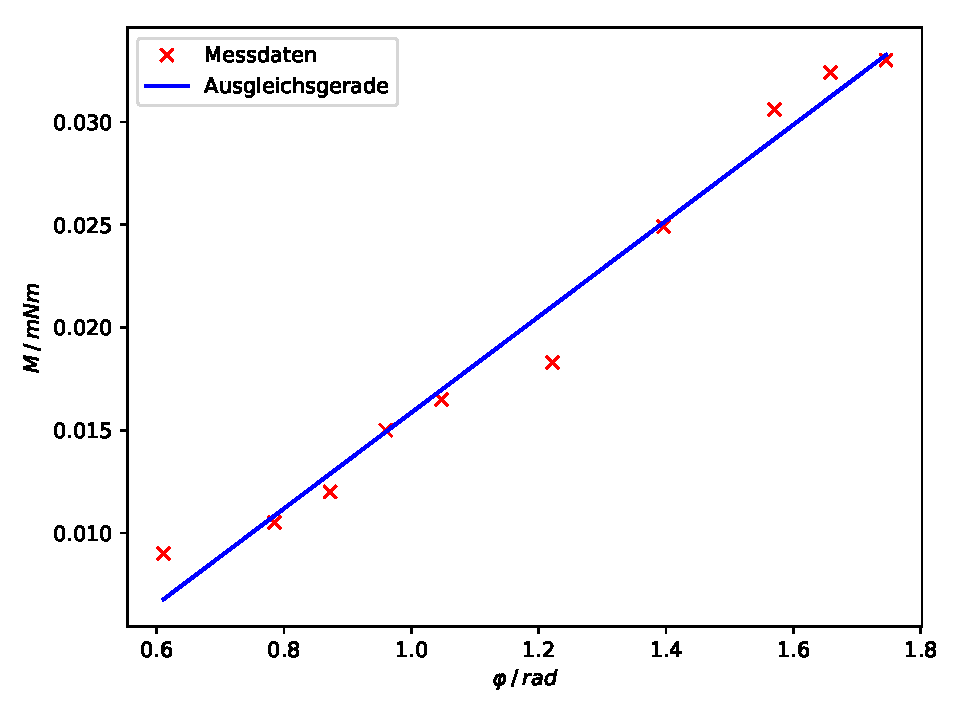
\includegraphics[scale=0.8]{content/plot1.pdf}
  \caption{Darstellung des Zusammenhanges zwischen dem Drehmoment und Winkel}
  \label{fig:plot1}
\end{figure}

Die Ausgleichsgerade ist gegeben mit $M(\varphi) = a\cdot \varphi + b$. Für die Regressionsparameter
ergibt sich: 

\begin{align*}
a &= \SI{23.34+-1.43}{\milli\newton\meter} \\
b &= \SI{-7.5+-1.78}{\milli\newton\meter}
\end{align*}

Der Steigungsfaktor $a$ entspricht dabei der Winkelrichtgröße $D$. Somit ergibt sich: 

\begin{equation*}
D = \SI{23.34+-1.43}{\milli\newton\meter}
\end{equation*}

\subsection{Bestimmung des Trägheitsmoments der Drillachse}

Zur Bestimmung des Eigenträgheitsmoments der Drillachse wird die Periodendauer $T$ in Abhängigkeit 
des Abstands $a$ der Gewichte zur Drillachse gemessen. Die erhaltenen Daten sind in Tabelle 
\ref{tab:Messdaten2} aufgeführt. Dabei ist $T$ die gemessene Dauer für 7 Perioden.

\begin{table}
\centering
\caption{Messwerte zum Trägheitsmoment der Drehachse}
\label{tab:Messdaten2}
\sisetup{table-format=2.1}
\begin{tabular}{c c c c c}
\toprule
$a \,/\, \si{\meter}$ & $a² \,/\, m²$ & $T\,/\, \si{\second}$ & $\frac{T}{7} \,/\, \si{\second}$ & $T² \,/\, s²$\\
\midrule
 0,2700 & 0,0729 & 57,93\,\pm 0,5 & 8,28\,\pm 0,071 & 68,49\,\pm 1,18\\
 0,2300 & 0,0529 & 50,30\,\pm 0,5 & 7,19\,\pm 0,071 & 51,63\,\pm 1,03\\
 0,2090 & 0,0437 & 46,89\,\pm 0,5 & 6,70\,\pm 0,071 & 44,87\,\pm 0,96\\
 0,1885 & 0,0355 & 43,00\,\pm 0,5 & 6,14\,\pm 0,071 & 37,73\,\pm 0,88\\
 0,1695 & 0,0287 & 40,10\,\pm 0,5 & 5,73\,\pm 0,071 & 32,82\,\pm 0,82\\
 0,1490 & 0,0222 & 35,72\,\pm 0,5 & 5,10\,\pm 0,071 & 26,04\,\pm 0,73\\
 0,1295 & 0,1677 & 32,58\,\pm 0,5 & 4,65\,\pm 0,071 & 21,66\,\pm 0,66\\
 0,1090 & 0,0119 & 28,85\,\pm 0,5 & 4,12\,\pm 0,071 & 16,99\,\pm 0,59\\
 0,0890 & 0,0079 & 25,49\,\pm 0,5 & 3,64\,\pm 0,071 & 13,26\,\pm 0,52\\
 0,0690 & 0,0048 & 22,36\,\pm 0,5 & 1,19\,\pm 0,071 & 10,20\,\pm 0,46\\
\bottomrule
\end{tabular}
\end{table}

Aus \eqref{eqn:Steiner} und \eqref{eqn:Periode} folgt der Zusammenhang: 

\begin{equation*}
T² = \underbrace{\frac{4\pi²m}{D}}_{\hat = s}\cdot a² + \underbrace{\frac{4\pi²}{D} I_\text{D}}_{\hat = b}
\label{eqn:Regression}
\end{equation*}

Mittels linearer Regression wird nun der als $b$ bezeichnete Parameter 
ermittelt und daraus das gesuchte Trägheitsmoment $I_\text{D}$ berechnet. Das 
Ergebnis ist in Abbildung \ref{fig:plot2} dargestellt. 

\begin{figure}
  \centering
  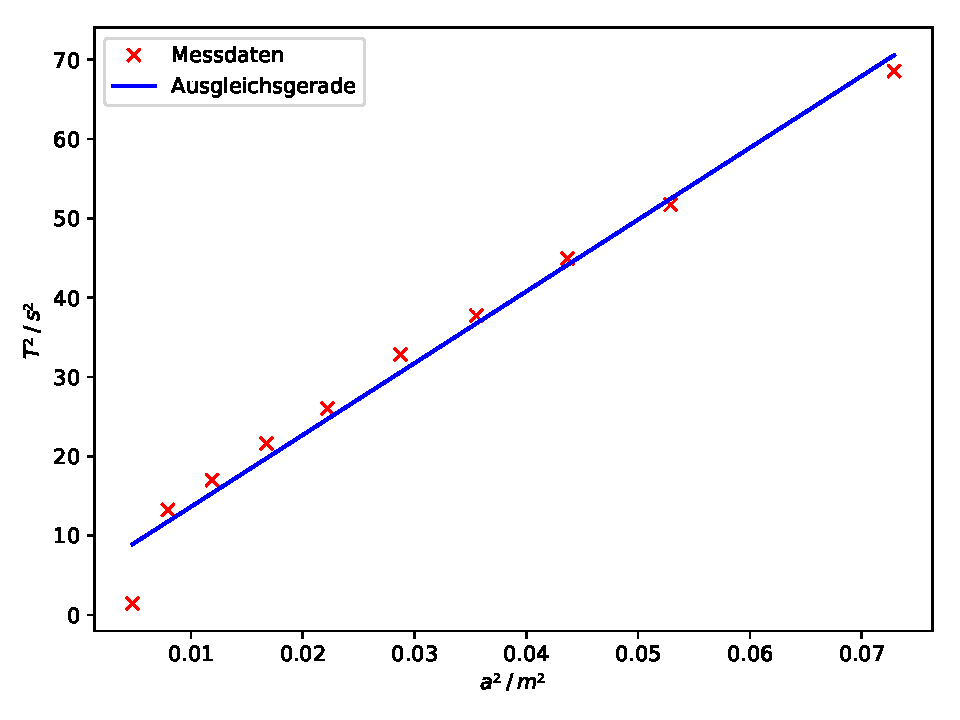
\includegraphics[scale=0.8]{content/plot2.pdf}
  \caption{$T²$ gegen $a²$ aufgetragen}
  \label{fig:plot2}
\end{figure}

Die Parameter der Ausgleichsgerade ergeben sich zu: 

\begin{align*}
s &= \SI{905.17+-54.89}{\second²\per\meter²},\\
b &= \SI{4.59+-1.99}{\second²}.
\end{align*}

Damit berechnet sich $I_\text{D}$ zu: 

\begin{equation*}
I_\text{D} = \frac{b\cdot D}{4\pi²} = \SI{2.7+-1.2e-3}{\kilo\gram\meter²}
\end{equation*}

Der statistische Fehler berechnet sich dabei mit der Gaußschenfehlerfortpflanzung 
zu: 

\begin{equation*}
\symup{\Delta} I_\text{D} = \sqrt{\left(\frac{\partial I_\text{D}}{\partial b}\cdot \symup{\Delta} b\right)²+\left(\frac{\partial I_\text{D}}{\partial D}\cdot \symup{\Delta} D\right)²}
= \sqrt{\left(\frac{D}{4\pi²}\cdot \symup{\Delta} b\right)²+\left(\frac{b}{4\pi²}\cdot \text{\Delta} D\right)²}.
\end{equation*}

\subsubsection{Verifikation des Satzes von Steiner}

Anhand der Daten, die zur Ermittelung des Eigenträgheitsmoments $I_\text{D}$ berechnet wurden, lässt sich der
Satz von Steiner verifizieren. Die verwendete Regressionsformel \eqref{eqn:Regression} folgt unter der
Annahme, das der Steiner'sche Satz gilt. Diese Formel fordert einen linearen Zusammenhang zwischen 
$T²$ und $a²$. Wie in Abbildung \ref{fig:plot2} zu erkennen ist, lässt sich dieser Zusammenhang 
bestätigen. Die Geradensteigung

\begin{equation*}
s = \SI{905.17+-54.89}{\second²\per\meter²}
\end{equation*}

passt ebenfalls zu dem theoretischen Wert, der sich ,mit der Gesamtmasse der Gewichte  $m = 2\cdot 
\SI{0.2218}{\kilo\gram}$ in die Definition von $s$ in Formel \eqref{eqn:Regression} eingesetzt, zu 
dem Wert:

\begin{equation*}
s_\text{theo} = \SI{750+-50}{\second²\per\meter²}
\end{equation*}

ergibt.
Dabei ist der Fehler des theoretischen Wertes gegeben durch:

\begin{equation*}
\symup{\Delta} s = \frac{-4\pi²m}{D²}.
\end{equation*}

\subsection{Trägheitsmomente zweier einfacher Körper}

Die zu untersuchenden Körper werden oben auf der Drillachse befestigt, zum Schwingen gebracht 
und die Periodendauer $T$ gemessen. Es werden zwei Körper untersucht: Ein Zylinder und eine Kugel.
Diese Körper besitzen folgende Maße: 

\begin{align*}
m_\text{Z} &= \SI{1005.9}{\gram},\\
d_\text{Z} &= \SI{7.95+-0.05}{\centi\meter},\\
m_\text{K} &= \SI{812.4}{\gram},\\
r_\text{K} &= \SI{7.5+-0.05}{\centi\meter}.
\end{align*}

Die ermittelten Periodendauer und Trägheitsmomente finden sich in Tabelle \ref{tab:Messdaten3}.

\begin{table}
\centering
\caption{Messwerte Kugel und Zylinder}
\label{tab:Messdaten3}
\sisetup{table-format=2.1}
\begin{tabular}{c c c c}
\toprule
\multicolumn{2}{c}{Zylinder} &  \multicolumn{2}{c}{Kugel} \\
\midrule
$T_\text{Z} \,/\, \si{\second}$ & $I_\text{Z} \,/\, \SI{1e-3}{\kilo\gram\meter²}$ & $T_\text{K}\,/\, \si{\second}$ & $I_\text{K} \,/\, \SI{1e-3}{\kilo\gram\meter²}$\\
\midrule
 1,21\,\pm 0,07 & 0,862\,\pm 0,115 & 1,73\,\pm 0,71 & 1,769\,\pm 0,182\\
 1,14\,\pm 0,07 & 0,770\,\pm 0,107 & 1,69\,\pm 0,71 & 1,691\,\pm 0,176\\
 1,15\,\pm 0,07 & 0,782\,\pm 0,108 & 1,73\,\pm 0,71 & 1,767\,\pm 0,182\\
 1,15\,\pm 0,07 & 0,782\,\pm 0,108 & 1,66\,\pm 0,71 & 1,629\,\pm 0,172\\
 1,16\,\pm 0,07 & 0,196\,\pm 0,109 & 1,69\,\pm 0,71 & 1,686\,\pm 0,176\\
\midrule
\multicolumn{2}{c}{$\bar{I_\text{Z}}= \SI{0.80+-0.07}{\kilo\gram\meter²}$} & \multicolumn{2}{c}{$\bar{I_\text{K}} = \SI{1.71+-0.12}{\kilo\gram\meter²}$} \\
\bottomrule
\end{tabular}
\end{table}

Dabei ergeben sich die Fehler der Trägheitsmomente zu: 

\begin{equation*}
\Delta I = \sqrt{\left(\frac{\partial I}{\partial T}\cdot \symup{\Delta} T\right)²+\left(\frac{\partial I}{\partial D}\cdot \symup{\Delta} D\right)²}
= \sqrt{\left(\frac{T D}{2\pi²}\cdot \symup{\Delta} T\right)²+\left(\frac{T²}{4\pi²}\cdot \symup{\Delta} D\right)²}
\end{equation*}

Nun werden die theoretischen Trägheitsmomente der beiden Körper berechnet, um die 
experimentell ermittelten Daten mit diesen zu vergleichen. Die Trägheitsmomente 
der Kugel bzw. des Zylinders werden hierbei mit den bekannten Formeln berechnet:

\begin{align*}
I_\text{K,theo} &= \frac{2}{5} mR²,\\
I_\text{Z,theo} &= \frac{1}{2} mR².
\end{align*}

Mit den Maßen der verwendeten Körper ergeben sich somit: 

\begin{align*}
I_\text{K,theo} &= \SI{1.828+-0.024}{\kilo\gram\meter²},\\
I_\text{Z,theo} &= \SI{0.795+-0.010}{\kilo\gram\meter²}.
\end{align*}

Die experimentell bestimmten Trägheitsmomente weichen von den theoretischen
Werten um $\SI{6.9}{\percent}$ bei der Kugel und um $\SI{0.625}{\percent}$ bei dem Zylinder ab.

\subsection{Trägheitsmoment einer Puppe in zwei Stellungen}
\subsubsection{Gemessene Trägheitsmomente}

Die beiden Stellungen der Puppe sind in Abbildung \ref{fig:Stellungen} dargestellt.

\begin{figure}
  \centering
  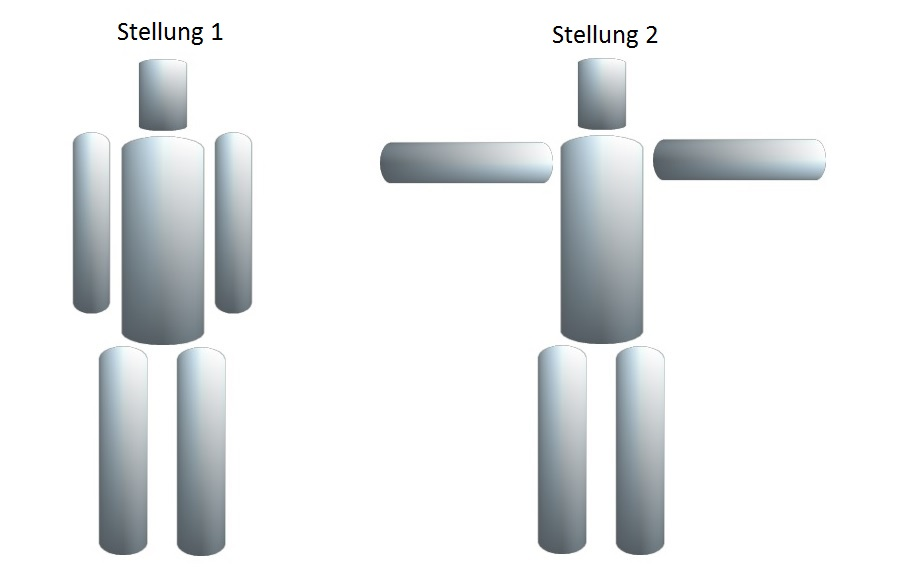
\includegraphics[scale=0.2]{content/Puppe_Stellungen.jpg}
  \caption{Stellungen der Puppe}
  \label{fig:Stellungen}
\end{figure}

Die Trägheitsmomente sollen durch eine Zeitmessung und das Umstellen der Formel \eqref{eqn:Periode} zu

\begin{equation}
  I = \frac{T^2 D} {4 \pi^2}
\end{equation}

bestimmt werden. In Tabelle \ref{tab:Periodendauer} sind die gemessenen Periodendauern $T_1$ für eine Puppe
in Stellung eins und zwei aufgelistet. Diese wurde für jeweils $7$ Schwingungen gemessen.  
Daraus ergeben sich die Trägheitsmomente $I_1$, $I_2$ für die Positionen 1 und 2 der Puppe.

\begin{align*}
  I_\text{1,mess} &= \SI{1.2+-0.2 e-4}{\kilo\gram\meter²},\\
  I_\text{2,mess} &= \SI{2.3+-0.3 e-4}{\kilo\gram\meter²}.
\end{align*}

\begin{table}
  \centering
  \caption{Messwerte der Periodendauern}
  \label{tab:Periodendauer}
  \sisetup{table-format=2.1}
  \begin{tabular}{c c c c}
  \toprule
  $T_1 \,/\, \si{\second}$ & $\frac{T_1}{7} \,/\, \si{\second}$ & 
  $T_2 \,/\, \si{\second}$ & $\frac{T_2}{7} \,/\, \si{\second}$ \\
  \midrule
   3,22\,\pm 0,5 & 0,46\,\pm 0,07 & 4,33\,\pm 0,5 & 0,62\,\pm 0,07 \\
   3,16\,\pm 0,5 & 0,45\,\pm 0,07 & 4,26\,\pm 0,5 & 0,61\,\pm 0,07 \\
   3,22\,\pm 0,5 & 0,46\,\pm 0,07 & 4,20\,\pm 0,5 & 0,60\,\pm 0,07 \\
   3,08\,\pm 0,5 & 0,44\,\pm 0,07 & 4,57\,\pm 0,5 & 0,65\,\pm 0,07 \\
   3,17\,\pm 0,5 & 0,45\,\pm 0,07 & 4,51\,\pm 0,5 & 0,64\,\pm 0,07 \\
  \bottomrule
  \end{tabular}
  \end{table}

  \subsubsection{Theoretische Trägheitsmomente}

  \begin{figure}
    \centering
    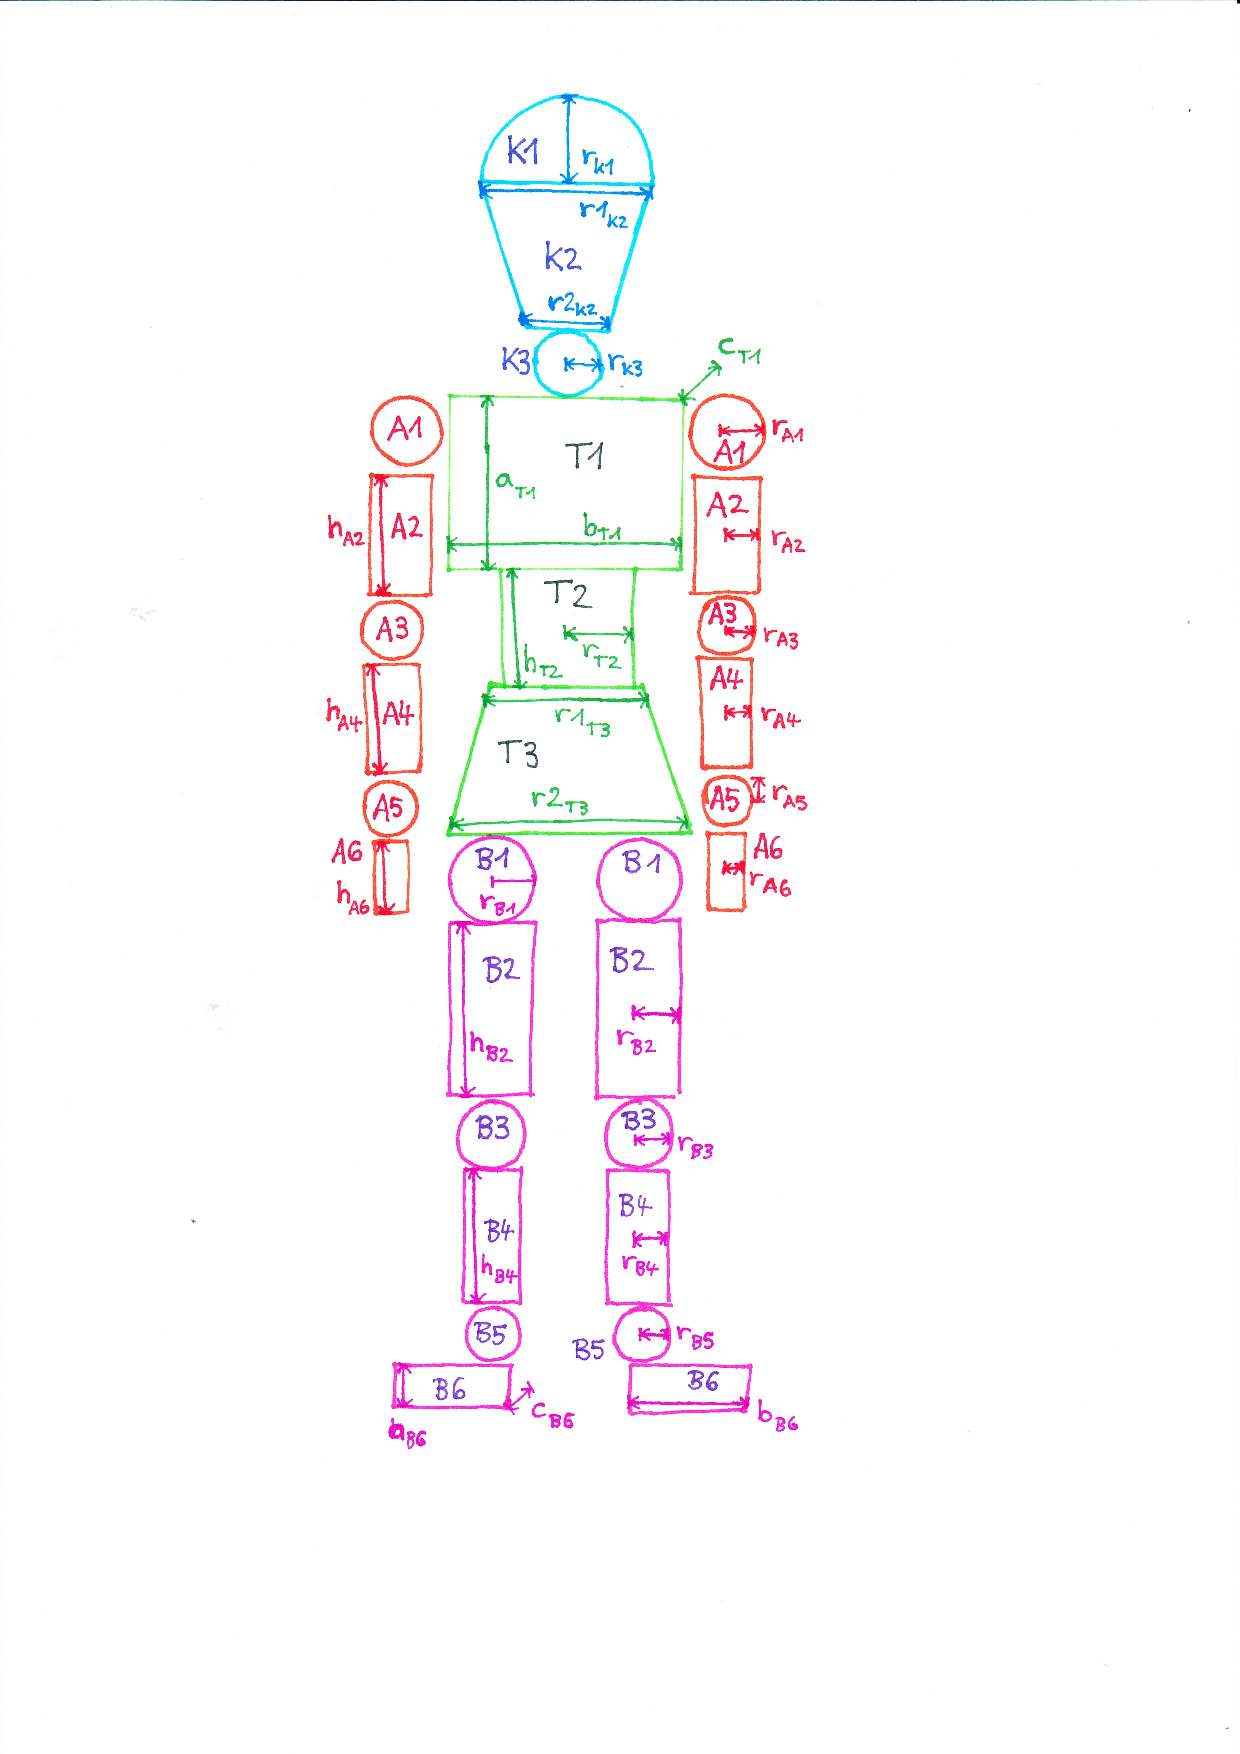
\includegraphics[scale=0.8]{content/Igor.pdf}
    \caption{Puppe mit anliegenden Armen, unterteilt in verschiedene
    geometrische Figuren}
    \label{fig:Igor}
  \end{figure}

  Wie in Abbildung \ref{fig:Igor} dargestellt, kann die Figur durch geometrische Figuren
  genähert werden. Dabei beschreiben die Figuren $K_\text{i}$ den Kopf, $T_\text{i}$ 
  den Torso, $A_\text{i}$ die Arme und $B_\text{i}$ die Beine.
  
  Die verwendeten geometrischen Figuren sind 
  (Halb-)Kugeln - als (Halb-)Kreise dargestellt und mit angegebenen Radien $r$ -, 
  Zylinder - als Rechtecke dargestellt und mit angegebenen Radien $r$ und Höhen $h$ -, 
  Quader - als Rechtecke dargestellt und mit angegebenen Seitenlängen $a$, $b$, $c$ -
  und Kegelstümpfe - als Trapeze dargestellt und mit angebenen Radien $r1$ und $r2$. 
  Die Abmessungen und resultierneden Volumina $V$ dieser Figuren sind in Tabelle
  \ref{tab:Abmessungen} aufgelistet. \\

\begin{table}
  \centering
  \caption{Abmessungen der Figuren}
  \label{tab:Abmessungen}
  \sisetup{table-format=2.1}
  \begin{tabular}{c c c c}
  \toprule
  $\text{Figur}$ & $\text{Abmessungen}$ & $\text{in } \si{\milli\meter}$ 
  & $V \,/\, \SI{e-5}{\meter³}$ \\
  \midrule
   K1 & $r_\text{K1} = $  & 16,00\,\pm 0,25 & 1,72\,\pm 0,08 \\
   K2 & $r1_\text{K2} = $ & 16,00\,\pm 0,25 & 2,35\,\pm 0,08 \\
      & $r2_\text{K2} = $ &  9,50\,\pm 0,25 & $ $ \\
      & $h_\text{K2} = $  & 45,50\,\pm 0,50 & $ $ \\
   K3 & $r_\text{K3} = $  &  8,00\,\pm 0,25 & 0,21\,\pm 0,02 \\
   T1 & $a_\text{T1} = $  & 48,70\,\pm 0,50 & 7,01\,\pm 0,15 \\
      & $b_\text{T1} = $  & 40,00\,\pm 0,50 & $ $ \\
      & $c_\text{T1} = $  & 36,00\,\pm 0,50 & $ $ \\
   T2 & $r_\text{T2} = $  & 12,85\,\pm 0,25 & 0,69\,\pm 0,04 \\
      & $h_\text{T2} = $  & 13,30\,\pm 0,50 & $ $ \\
   T3 & $r1_\text{T3} = $ & 15,15\,\pm 0,25 & 3,41\,\pm 0,08 \\
      & $r2_\text{T3} = $ & 19,70\,\pm 0,25 & $ $ \\
      & $h_\text{T3} = $  & 35,50\,\pm 0,50 & $ $ \\
   A1 & $r_\text{A1} = $  &  8,00\,\pm 0,25 & 0,21\,\pm 0,02 \\
   A2 & $r_\text{A2} = $  &  8,00\,\pm 0,25 & 0,86\,\pm 0,05 \\
      & $h_\text{A2} = $  & 42,80\,\pm 0,50 & $ $ \\
   A3 & $r_\text{A3} = $  &  5,80\,\pm 0,25 & 0,08\,\pm 0,01 \\
   A4 & $r_\text{A4} = $  &  7,15\,\pm 0,25 & 0,69\,\pm 0,05 \\
      & $h_\text{A4} = $  & 42,80\,\pm 0,50 & $ $ \\
   A5 & $r_\text{A5} = $  &  4,75\,\pm 0,25 & 0,05\,\pm 0,01 \\
   A6 & $r_\text{A6} = $  &  7,75\,\pm 0,25 & 0,50\,\pm 0,03 \\
      & $h_\text{A6} = $  & 26,70\,\pm 0,50 & $ $ \\
   B1 & $r_\text{B1} = $  &  8,40\,\pm 0,25 & 0,25\,\pm 0,02 \\
   B2 & $r_\text{B2} = $  &  9,10\,\pm 0,25 & 1,47\,\pm 0,08 \\
      & $h_\text{B2} = $  & 56,40\,\pm 0,50 & $ $ \\
   B3 & $r_\text{B3} = $  &  6,25\,\pm 0,25 & 0,10\,\pm 0,01 \\
   B4 & $r_\text{B4} = $  &  7,35\,\pm 0,25 & 1,13\,\pm 0,08 \\
      & $h_\text{B4} = $  & 66,30\,\pm 0,50 & $ $ \\
   B5 & $r_\text{B5} = $  &  4,60\,\pm 0,25 & 0,04\,\pm 0,01 \\
   B6 & $a_\text{B6} = $  &  5,40\,\pm 0,25 & 0,25\,\pm 0,02 \\
      & $b_\text{B6} = $  & 42,30\,\pm 0,50 & $ $ \\
      & $c_\text{B6} = $  & 10,80\,\pm 0,50 & $ $ \\
  \bottomrule
  \end{tabular}
  \end{table}

  Die Volumina ergeben sich nach den Formeln in Tabelle \ref{tab:Formeln}.
  Zur Massenbestimmung der einzelnen Bestandteile werden die Teilvolumina $V_\text{i}$ 
  zum Gesamtvolumen $V = \SI{26.63e-5}{\meter³}$ aufsummiert.
  Dabei ist darauf zu achten, dass die Komponenten der Arme und Beine jeweils doppelt
  vorhanden sind. Mit der Gesamtmasse
  $m = \SI{0.1626}{\kilo\gram}$ ergibt sich die Dichte

  \begin{equation}
    \rho = \frac{m}{V} = \SI{611+-8}{\kilo\gram\per\meter³}.
    \label{eqn:Dichte}
  \end{equation}

  Wird von einer homogenen Dichte ausgegangen, berechnen sich die Massen der einzelnen
  Komponenten nach Umstellen von \eqref{eqn:Dichte} zu

  \begin{equation}
    m_\text{i} = \rho \cdot V.
  \end{equation}

  Mit diesen Einzelmassen lassen sich nach Tabelle \ref{tab:Formeln} die Trägheitsmomente
  der einzelnen Körper bestimmen, welche in Tabelle \ref{tab:Trägheit} aufgelistet sind.

  \begin{table}
    \centering
    \caption{Volumina und Trägheitsmomente verschiedener Figuren}
    \label{tab:Formeln}
    \sisetup{table-format=2.1}
    \begin{tabular}{c c c}
    \toprule
    $\text{Figur}$ & $V$ & $I$ \\
    \midrule
     $\text{Kugel}$         & $ = \frac{4}{3} \pi r^3 $ & $ = \frac{2}{5} m r^2 $ \\                        
     $\text{Halbkugel}$     & $ = \frac{2}{3} \pi r^3 $ & $ = \frac{2}{5} m r^2 $ \\
     $\text{Zylinder um h}$ & $ = \pi r^2 \cdot h $     & $ = \frac{1}{2} m r^2 $ \\
     $\text{Zylinder um r}$ & $ = \pi r^2 \cdot h $     & $ = \frac{m}{4} \left(r^2 + \frac{h^2}{3} \right)$ \\
     $\text{Quader}$        & $ = a\cdot b \cdot c$     & $ = \frac{3}{10} m \frac{r_\text{g}^5 - r_\text{k}^5}{r_\text{g}^3 - r_\text{k}^3}$ \\
     $\text{Kegelstumpf}$   & $ = \frac{h \pi}{3}\cdot \left(r_\text{g}^2 + r_\text{g} r_\text{k}
      + r_\text{k}^2 \right) $ & $ = \frac{1}{12} m \left(b^2 + c^2 \right)$ \\
    \bottomrule
    \end{tabular}
    \end{table}

    \begin{table}
      \centering
      \caption{Trägheitsmomente}
      \label{tab:Trägheit}
      \sisetup{table-format=2.1}
      \begin{tabular}{c c c c}
      \toprule
      $\text{Figur}$ & $I_\text{i} \,/\, \SI{e-7}{\kilo\gram\meter²}$ & $a_\text{i} \,/\, \si{\milli\meter}$ 
      & $I_\text{i,Steiner} \,/\, \SI{e-7}{\kilo\gram\meter²}$ \\
      \midrule
       K1 &  10,70\,\pm 0,80                  & -              & - \\
       K2 &  12,90\,\pm 0,70                  & -              & - \\
       K3 &   0,30\,\pm 0,05                  & -              & - \\
       T1 & 103,00\,\pm 4,00                  & -              & - \\
       T2 &   3,50\,\pm 0,30                  & -              & - \\
       T3 &  32,50\,\pm 1,40                  & -              & - \\
       B1 &   0,43\,\pm 0,06                  &  12,5\,\pm 1,5 &   2,80\,\pm  0,60 \\
       B2 &   3,70\,\pm 0,04                  &  16,0\,\pm 1,5 &  27,00\,\pm  5,00 \\
       B3 &   0,10\,\pm 0,02                  &  13,0\,\pm 1,5 &   1,15\,\pm  0,28 \\
       B4 &   1,86\,\pm 0,24                  &  19,0\,\pm 1,5 &  27,00\,\pm  4,00 \\
       B5 &   0,02\,\pm 0,01                  &  14,0\,\pm 1,5 &   0,51\,\pm  0,13 \\
       B6 &   2,39\,\pm 0,25                  &  15,0\,\pm 1,5 &   5,80\,\pm  0,90 \\
       A1 &   0,34\,\pm 0,05                  &  30,0\,\pm 1,5 &  12,10\,\pm  1,60 \\
       A2 &   1,68\,\pm 0,21                  &  27,5\,\pm 1,5 &  41,00\,\pm  5,00 \\
       A3 &   0,07\,\pm 0,01                  &  27,5\,\pm 1,5 &   3,80\,\pm  0,60 \\
       A4 &   1,07\,\pm 0,15                  &  30,0\,\pm 1,5 &  39,00\,\pm  5,00 \\
       A5 &   0,03\,\pm 0,01                  &  30,0\,\pm 1,5 &   2,50\,\pm  0,50 \\
       A6 &   0,92\,\pm 0,12                  &  30,0\,\pm 1,5 &  28,60\,\pm  3,40 \\
       $ \text{A1}_\text{gestreckt} $ &  0,34\,\pm 0,05 &  30,0\,\pm 1,5 &  12,10\,\pm  1,60 \\
       $ \text{A2}_\text{gestreckt} $ &  8,90\,\pm 0,06 &  59,0\,\pm 1,5 & 192,00\,\pm 15,00 \\
       $ \text{A3}_\text{gestreckt} $ &  0,07\,\pm 0,01 &  83,0\,\pm 1,5 &  34,00\,\pm  5,00 \\
       $ \text{A4}_\text{gestreckt} $ &  6,90\,\pm 0,60 & 108,0\,\pm 1,5 & 500,00\,\pm 40,00 \\
       $ \text{A5}_\text{gestreckt} $ &  0,03\,\pm 0,01 & 131,0\,\pm 1,5 &  47,00\,\pm  8,00 \\
       $ \text{A6}_\text{gestreckt} $ &  2,29\,\pm 0,21 & 146,5\,\pm 1,5 & 660,00\,\pm 50,00 \\
      \bottomrule
      \end{tabular}
      \end{table}

      Da die Schwerpunkte der Komponenten der Arme und Beine nicht auf der Drehachse liegen,
      muss für diese der Satz von Steiner nach \eqref{eqn:Steiner} beachtet werden. 
      Nach diesem addiert sich zu jedem Trägheitsmoment das Produkt von Masse $m_\text{i}$ und
      Abstand zwischen Schwerpunkt und Drehachse  zum Quadrat $a_\text{i}^2$ zum Trägheitsmoment
      auf der Drehachse. Somit ergeben sich nach Tabelle \ref{tab:Trägheit} für die Komponenten
      mit Abständen $a_\text{i}$ die Trägheitsmomente $I_\text{i,Steiner}$.
      Diese summieren sich für Position 1 und 2 zu

      \begin{align*}
        I_\text{1,theo} &= \SI{5.45+-0.19 e-5}{\kilo\gram\meter²},\\
        I_\text{2,theo} &= \SI{31.8+-1.2 e-5}{\kilo\gram\meter²}.
      \end{align*}